\documentclass[11pt]{article}
\usepackage[margin=1in]{geometry}
\usepackage[T1]{fontenc}
\usepackage{lmodern}
\usepackage{amsmath,amssymb}
\usepackage{booktabs}
\usepackage{enumitem}
\usepackage{xcolor}
\usepackage{tikz}
\usetikzlibrary{positioning,arrows.meta,calc}
\usepackage[most]{tcolorbox}
\usepackage{listings}
\usepackage[hidelinks]{hyperref}
\usepackage{microtype}

\setlist{itemsep=2pt,topsep=3pt}
\setlength{\parskip}{5pt}
\setlength{\parindent}{0pt}

\definecolor{iceblue}{RGB}{30,100,200}
\definecolor{icebg}{RGB}{235,243,255}
\definecolor{keybg}{RGB}{255,248,225}

\newtcolorbox{idea}[1]{colback=icebg,colframe=iceblue,fonttitle=\bfseries,title=#1,boxrule=0.6pt,arc=2pt}
\newtcolorbox{example}[1]{colback=keybg,colframe=orange!70!black,fonttitle=\bfseries,title=#1,boxrule=0.6pt,arc=2pt}

\lstset{basicstyle=\ttfamily\footnotesize,keywordstyle=\color{iceblue}\bfseries,
  commentstyle=\color{gray}\itshape,frame=single,framerule=0.4pt,rulecolor=\color{gray!60},
  backgroundcolor=\color{gray!5},columns=fullflexible,keepspaces=true,language=Python,
  showstringspaces=false,xleftmargin=4pt,xrightmargin=4pt,breaklines=true}

\newcommand{\R}{\mathbb{R}}
\newcommand{\norm}{\mathrm{RMSNorm}}

\title{\textbf{How ICE Is Injected Into the Model}\\[3pt]\large A step-by-step explanation with formulas}
\author{Phung Gia Huy}
\date{October 2026}

\begin{document}
\maketitle

\begin{idea}{The whole idea in three sentences}
A \textbf{fixed (non-learned) lookup} finds where the last $n$ tokens appeared earlier and reports the token that came next.
The model \textbf{learns how much to trust} that hint, using two small learned modules: one inside the network and one at the output.
\textbf{ICE-dropout} sometimes hides the hint during training, so attention does not become lazy.
\end{idea}

Throughout, we use the model from the proposal: a hybrid with 16 layers, hidden size $d = 768$ and vocabulary size $V \approx 32{,}000$.

%=====================================================================
\section{Where ICE plugs into the model}

ICE touches the model in exactly \textbf{two places}. Everything else is a normal hybrid model.

\begin{center}
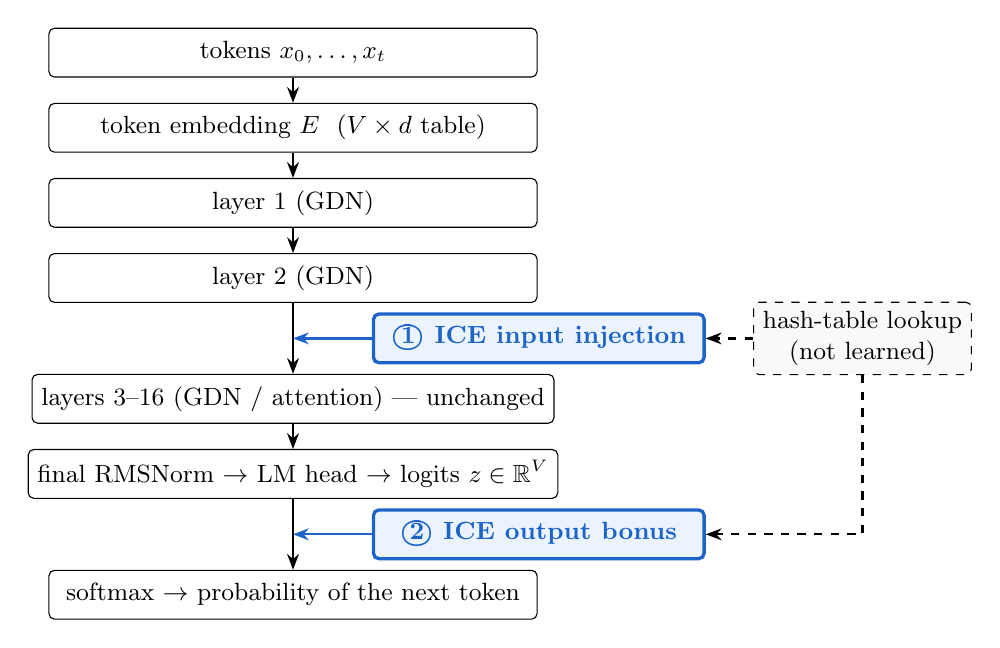
\begin{tikzpicture}[
  box/.style={draw,rounded corners=2pt,minimum width=6.2cm,minimum height=0.62cm,font=\small,fill=white},
  ice/.style={draw=iceblue,very thick,rounded corners=2pt,minimum width=4.2cm,minimum height=0.62cm,font=\small\bfseries,fill=icebg,text=iceblue},
  arr/.style={-{Stealth[length=2mm]},thick},
  node distance=0.32cm]
  \node[box] (tok) {tokens $x_0, \dots, x_t$};
  \node[box,below=of tok] (emb) {token embedding $E$ \ ($V \times d$ table)};
  \node[box,below=of emb] (l1) {layer 1 (GDN)};
  \node[box,below=of l1] (l2) {layer 2 (GDN)};
  \node[box,below=0.9cm of l2] (l3) {layers 3--16 (GDN / attention) --- unchanged};
  \node[box,below=of l3] (head) {final RMSNorm $\to$ LM head $\to$ logits $z \in \R^V$};
  \node[box,below=0.9cm of head] (soft) {softmax $\to$ probability of the next token};
  \foreach \a/\b in {tok/emb,emb/l1,l1/l2,l2/l3,l3/head,head/soft} \draw[arr] (\a) -- (\b);

  \node[ice,right=1.0cm of $(l2)!0.5!(l3)$] (icein) {\textcircled{1} ICE input injection};
  \node[ice,right=1.0cm of $(head)!0.5!(soft)$] (iceout) {\textcircled{2} ICE output bonus};
  \draw[arr,iceblue] (icein.west) -- ($(l2)!0.5!(l3)$);
  \draw[arr,iceblue] (iceout.west) -- ($(head)!0.5!(soft)$);

  \node[draw,dashed,rounded corners=2pt,font=\small,align=center,fill=gray!5,right=0.6cm of icein] (lookup)
     {hash-table lookup\\(not learned)};
  \draw[arr,dashed] (lookup.west) -- (icein.east);
  \draw[arr,dashed] (lookup.south) |- (iceout.east);
\end{tikzpicture}
\end{center}

\begin{itemize}
  \item \textcircled{1} \textbf{Input injection}, after layer 2: the hints are added to the hidden state, so layers 3--16 can use them.
  \item \textcircled{2} \textbf{Output bonus}, at the logits: the copied token gets extra score.
\end{itemize}

%=====================================================================
\section{Step 0: what the lookup returns (no learning)}

At position $t$ the model must predict $x_{t+1}$. For each order $n \in \{1,2,3,4,6,8\}$, the hash table looks for the most recent earlier position $p < t$ where the same last $n$ tokens appeared, and returns four integers:

\begin{center}
\begin{tabular}{@{}cl@{}}
\toprule
Symbol & Meaning \\
\midrule
$m_n \in \{0,1\}$ & 1 if a match exists, 0 if not \\
$s_n$ & the \emph{successor}: the token that came after the earlier match, $x_{p+1}$ \\
$\ell_n$ & the match length (as a bucket) \\
$\delta_n$ & how far back the match is: $\lfloor \log_2(t-p) \rfloor$ \\
\bottomrule
\end{tabular}
\end{center}

\begin{example}{Example}
Text so far: \quad \texttt{\dots\ user = get\_user(req, id) \dots\ user = get\_user(req,} \quad $\to$ \ ?

\begin{center}
\begin{tabular}{@{}cccc@{}}
\toprule
order $n$ & match? $m_n$ & successor $s_n$ & distance \\
\midrule
8 & 1 & \texttt{id} & 512 tokens back \\
4 & 1 & \texttt{id} & 512 tokens back \\
1 & 1 & \texttt{self} & 3 tokens back (another call) \\
\bottomrule
\end{tabular}
\end{center}
The long matches are reliable; the 1-token match is noise. The model must learn this.
\end{example}

Because $p < t$, the successor $x_{p+1}$ is always a token the model has \emph{already seen}. ICE never looks at the future.

%=====================================================================
\section{Injection \textcircled{1}: adding the hints inside the network}

Let $h_t \in \R^{768}$ be the hidden state of token $t$ after layer 2.

\subsection*{Step 1 --- turn each hint into a vector}
\[
\boxed{\, f_n \;=\; W_n \, E[s_n] \;+\; L[\ell_n] \;+\; D[\delta_n] \,}
\]
\begin{itemize}
  \item $E[s_n] \in \R^{768}$: the embedding of the hinted token. It is the \textbf{same table} the model uses for its input words, so the hint ``speaks the model's language'' from the start.
  \item $W_n \in \R^{768 \times 768}$: a learned matrix, one per order. An 8-gram hint and a 1-gram hint can carry different messages.
  \item $L[\ell_n]$, $D[\delta_n] \in \R^{768}$: small learned vectors for ``how long the match was'' and ``how far back it was''.
\end{itemize}
In words, $f_n$ says: \emph{``the hint is token \texttt{id}, from an 8-token match, 512 tokens back.''}

\subsection*{Step 2 --- decide how much to trust it (the gate)}
\[
\boxed{\, g_n \;=\; \sigma\!\left( \frac{\big\langle \norm(h_t),\ \norm(f_n) \big\rangle}{\sqrt{d}} \right) \in (0,1) \,}
\]
\begin{itemize}
  \item The dot product $\langle\cdot,\cdot\rangle$ measures \textbf{how well the hint agrees with what the model currently thinks}.
  \item If the context suggests ``we are inside a repeated function call'', $h_t$ and $f_n$ point in similar directions, so the dot product is large and $g_n \approx 1$.
  \item If the hint makes no sense here, they disagree and $g_n \approx 0$.
  \item $\sigma$ (the sigmoid) squashes the result into $(0,1)$, like a \textbf{volume knob}.
  \item RMSNorm puts both vectors on the same scale, so the gate depends on \emph{direction} (agreement), not on size.
\end{itemize}

\subsection*{Step 3 --- add the gated hints to the hidden state}
\[
\boxed{\, h_t \;\leftarrow\; h_t \;+\; \sum_{n} m_n \, g_n \, f_n \,}
\]
Orders with no match have $m_n = 0$ and add nothing. Layers 3--16 then run \textbf{unchanged} on the enriched $h_t$: they can use the hint, combine it with what attention finds, or ignore it.

\begin{example}{Example (continued)}
Suppose the learned gates give $g_8 = 0.9$, \ $g_4 = 0.8$, \ $g_1 = 0.05$. Then
\[
h_t \leftarrow h_t + 0.9\, f_8 + 0.8\, f_4 + 0.05\, f_1 ,
\]
so the model mostly ``hears'' the reliable 8-gram and 4-gram hints and almost ignores the 1-gram hint.
\end{example}

%=====================================================================
\section{Injection \textcircled{2}: the copy bonus at the output}

After the last layer, the model computes its normal logits (one score per vocabulary token):
\[
z \;=\; W_{\text{out}}\, \norm\big(h_t^{(16)}\big) \;\in\; \R^{V}.
\]
Let $s^*$ be the successor from the \textbf{longest} match (here \texttt{id}). ICE adds a learned bonus to that single entry:
\[
\boxed{\, \lambda_t = \mathrm{softplus}\!\Big( w^\top \norm\big(h_t^{(16)}\big) + b[\ell^*] \Big) \ \ge 0, \qquad z[s^*] \;\leftarrow\; z[s^*] + \lambda_t \,}
\]
\begin{itemize}
  \item $w \in \R^{768}$ and $b$ (one number per match-length bucket) are learned.
  \item $\mathrm{softplus}(u) = \log(1+e^u)$ is always $\ge 0$: ICE can only \emph{push up} the hinted token, never push it down.
  \item $\lambda_t$ is the model's \textbf{copy confidence}, recomputed at every token.
  \item Initialization: $w = 0$, $b = -2$, so $\lambda_t \approx 0.13$ at the start and training begins close to a model without ICE.
\end{itemize}
The next-token probability is then the usual $p = \mathrm{softmax}(z)$.

\begin{example}{Numeric example}
\begin{center}
\begin{tabular}{@{}lcccc@{}}
\toprule
token & logit (no ICE) & prob.\ (no ICE) & logit with $\lambda_t = 2$ & prob.\ with ICE \\
\midrule
\texttt{id}      & 3.0 & 0.42 & \textbf{5.0} & \textbf{0.84} \\
\texttt{user\_id} & 2.8 & 0.34 & 2.8 & 0.09 \\
\texttt{name}    & 2.0 & 0.15 & 2.0 & 0.04 \\
others           & ---  & 0.09 & --- & 0.02 \\
\bottomrule
\end{tabular}
\end{center}
With a confident bonus ($\lambda_t = 2$), the probability of \texttt{id} doubles. With low confidence ($\lambda_t \approx 0$), nothing changes.
\end{example}

%=====================================================================
\section{How ICE learns: it is just the normal training loss}

ICE needs \textbf{no extra loss and no labels}. The model is trained with ordinary next-token prediction:
\[
\mathcal{L} = -\log p(x_{t+1}).
\]

\subsection*{The copy bonus (cleanest case)}
For a softmax, the gradient of the loss with respect to the bonus is
\[
\boxed{\, \frac{\partial \mathcal{L}}{\partial \lambda_t} \;=\; p(s^*) \;-\; \mathbf{1}\big[\, s^* = x_{t+1} \,\big] \,}
\]
\begin{center}
\begin{tabular}{@{}lll@{}}
\toprule
Situation & Gradient & What training does \\
\midrule
Hint correct ($s^* = x_{t+1}$) & $p(s^*) - 1 < 0$ & \textbf{increases} $\lambda$ here: ``trust more'' \\
Hint wrong ($s^* \ne x_{t+1}$) & $p(s^*) > 0$ & \textbf{decreases} $\lambda$ here: ``trust less'' \\
\bottomrule
\end{tabular}
\end{center}
Because $\lambda_t$ is computed from the hidden state $h_t$ and the match length, the updates to $w$ and $b$ teach the model \emph{in which situations} to trust the hint: long matches, code, repeated function calls, and so on.

\subsection*{The input gate}
By the chain rule,
\[
\frac{\partial \mathcal{L}}{\partial g_n} \;=\; \Big\langle \frac{\partial \mathcal{L}}{\partial h_t},\ m_n f_n \Big\rangle .
\]
If adding the hint $f_n$ moves $h_t$ in a direction that lowers the loss, the gate opens more; otherwise it closes. The matrices $W_n$, the tables $L$ and $D$, and the norms are updated at the same time, so the hint vectors themselves become more useful.

\begin{example}{What the model ends up learning (nobody writes these rules)}
\begin{itemize}
  \item ``An 8-token match inside code is almost always right'' $\Rightarrow$ large $g_8$ and large $\lambda$.
  \item ``A 1-token match is nearly random'' $\Rightarrow$ $g_1 \approx 0$.
  \item ``A match right after \texttt{range(} is unreliable'' $\Rightarrow$ small $\lambda$ there.
\end{itemize}
\end{example}

%=====================================================================
\section{ICE-dropout}

\subsection*{The problem: ``lookup laziness''}
If the hint is always available, many tokens can be predicted just by copying it. The full-attention layers then get little reason to learn \emph{retrieval}. But ICE only handles \textbf{exact} repeats. When the text says the same thing in different words (``the blue door's code is 4721'' \dots\ ``what number opens the door that is blue?''), the hint is useless, and a model whose attention never learned retrieval fails.

This is like a student who always does homework with the answer key: high scores in practice, failure in the exam.

\subsection*{The fix, as a formula}
For each training \textbf{sequence}, flip one coin $k \sim \mathrm{Bernoulli}(0.8)$:
$k = 1$ (ICE on) 80\% of the time, $k = 0$ (ICE off) 20\% of the time. Multiply both injections by $k$:
\[
\boxed{\, h_t \;\leftarrow\; h_t + k \sum_{n} m_n\, g_n\, f_n, \qquad z[s^*] \;\leftarrow\; z[s^*] + k\, \lambda_t \,}
\]
\begin{itemize}
  \item When $k = 0$, the model is a plain hybrid for that whole text, so attention \emph{must} find the information itself and keeps learning retrieval.
  \item \textbf{At inference, $k = 1$ always.}
  \item The coin is per \textbf{sequence}, not per token, so attention must do the job across an entire text.
  \item Normal dropout rescales by $1/(1-p)$; we do not, because the gates already learn how loud the hint should be.
\end{itemize}

%=====================================================================
\section{Code sketch (PyTorch)}

\begin{lstlisting}
class ICEInput(nn.Module):                         # injection 1, after layer 2
    def __init__(self, d, n_orders=6, n_len=8, n_dist=16):
        super().__init__()
        self.W = nn.ModuleList([nn.Linear(d, d, bias=False) for _ in range(n_orders)])
        self.L, self.D = nn.Embedding(n_len, d), nn.Embedding(n_dist, d)
        self.norm_h, self.norm_f = nn.RMSNorm(d), nn.RMSNorm(d)

    def forward(self, h, tok_emb, succ, len_b, dist_b, k):
        # h: [B,T,d]; succ/len_b/dist_b: [B,T,N] ints (succ = -1 if no match); k: [B] in {0,1}
        m = (succ >= 0).float()                                  # m_n
        e = tok_emb(succ.clamp(min=0))                           # E[s_n]
        f = torch.stack([self.W[n](e[:, :, n]) for n in range(len(self.W))], dim=2)
        f = f + self.L(len_b) + self.D(dist_b)                   # f_n
        g = torch.sigmoid((self.norm_h(h).unsqueeze(2) * self.norm_f(f)).sum(-1)
                          / h.shape[-1] ** 0.5)                  # g_n
        add = ((m * g).unsqueeze(-1) * f).sum(dim=2)             # sum_n m_n g_n f_n
        return h + k[:, None, None] * add                        # ICE-dropout via k

class ICEOutput(nn.Module):                        # injection 2, at the logits
    def __init__(self, d, n_len=8):
        super().__init__()
        self.w, self.b, self.norm = nn.Linear(d, 1), nn.Embedding(n_len, 1), nn.RMSNorm(d)
        nn.init.zeros_(self.w.weight); nn.init.constant_(self.b.weight, -2.0)

    def forward(self, logits, h_last, s_star, len_star, k):
        lam = F.softplus(self.w(self.norm(h_last)) + self.b(len_star.clamp(min=0))).squeeze(-1)
        lam = lam * (s_star >= 0) * k[:, None]                   # no match or dropped -> 0
        return logits.scatter_add(-1, s_star.clamp(min=0).unsqueeze(-1), lam.unsqueeze(-1))
\end{lstlisting}

In the model's forward pass: \texttt{h = ice\_in(h, embed, \dots)} right after layer 2, and \texttt{logits = ice\_out(logits, h\_final, \dots)} right before the loss.

%=====================================================================
\section{Summary}

\begin{center}
\renewcommand{\arraystretch}{1.25}\small
\begin{tabular}{@{}llcl@{}}
\toprule
Piece & Formula & Learned? & Job \\
\midrule
Lookup & $m_n, s_n, \ell_n, \delta_n$ from a hash table & no & find exact repeats \\
Hint vector & $f_n = W_n E[s_n] + L[\ell_n] + D[\delta_n]$ & yes & describe the hint \\
Gate & $g_n = \sigma\big(\langle \norm\, h_t, \norm\, f_n \rangle / \sqrt d\big)$ & yes & how much to listen \\
Input injection & $h_t \leftarrow h_t + k \sum_n m_n g_n f_n$ & --- & give hints to layers 3--16 \\
Copy bonus & $z[s^*] \mathrel{+}= k\, \mathrm{softplus}(w^\top h + b[\ell^*])$ & yes & push up the copied token \\
ICE-dropout & $k \sim \mathrm{Bernoulli}(0.8)$; $k = 1$ at test time & --- & keep attention learning \\
\bottomrule
\end{tabular}
\end{center}

\textbf{Extra parameters:} about 4M (mostly the six $768 \times 768$ matrices $W_n$), roughly 3\% of the 140M model.
\textbf{Extra memory at inference:} about 100 bytes per token (token IDs and hash-table entries), versus 2--3\,KB per token for one full-attention layer.

\end{document}
